%
% CMPT 379: Principles of Compiler Design - A Course Overview
% Section: Parsing Algorithms: Bottom-Up
%
% Author: Jeffrey Leung
%

\section{Parsing Algorithms: Bottom-Up}
	\label{sec:parsing-algorithms-bottom-up}

\subsection{Introduction}
	\label{subsec:parsing-algorithms-bottom-up:introduction}
\begin{easylist}

& \textbf{Bottom-up parsing:} Reduction of a string of terminal symbols to the start symbol
	&& Simulates a reversed rightmost derivation (see \textit{shift-reduce parsing})

& \textbf{LR(k) parsing:} Bottom-up parsing derivation which parses \textbf{L}eft-to-right to create a \textbf{R}ightmost derivation with $k$ (usually 1) tokens of lookahead
	&& Actions:
		&&& Shift ($f: u \rightarrow a$)
		&&& Reduce ($f: \textrm{ lookup production  } x \rightarrow y_1 \dotsc y_n$)
		&&& Accept
		&&& Error

& \textbf{Dotted rule:} Parser state consisting of a single production rule and a dot ($\bullet$) where the parser currently is at
	&& Notation: $A \rightarrow B \bullet C$
	&& All symbols to the left of the dot have been read; all symbols to the right of the dot are predicted
	&& \textbf{Configuration/itemset/state:} Set of dotted rules which are all possible productions given an in-progress parse

		&&& E.g. Given a set of production rules and a dotted rule, the resulting configuration set is given in table~\ref{tab:config-set}

\end{easylist}
\begin{figure}[!htb]
	\caption{Configuration Set Example}
	\label{tab:config-set}
	\begin{center}
		\begin{tabular}{ r | l }
			Production Rules
			& $T \rightarrow F$ \\
			& $T \rightarrow T*F$ \\
			& $F \rightarrow id$ \\
			& $F \rightarrow (T)$ \\
			\hline
			Dotted Rule
			& $T \rightarrow T * \bullet F$ \\
			\hline
			\hline
			$closure(T \rightarrow T * \bullet F)$
			& $T \rightarrow T * \bullet F$ \\
			(Configuration set)
			& $F \rightarrow \bullet (T)$ \\
			& $F \rightarrow \bullet id$
		\end{tabular}
	\end{center}
\end{figure}
\begin{easylist}

& \textbf{Action/Goto (parsing) table:} Set of states and transitions which provides a programmatic method to parse an input
	&& Notations:
		&&& $\textrm{action}[s, a]; a \in T$ where $T$ is the set of terminal states
		&&& $\textrm{goto}[s, X]; X \in N$ where $N$ is the set of non-terminal states

	&& Layout: See table~\ref{tab:layout-action-table}

\end{easylist}
\begin{figure}[!htb]
	\caption{Layout of an action/goto table}
	\label{tab:layout-action-table}
	\begin{center}
		\begin{tabular}{ l | l l | l }
			\textbf{State} & \textbf{Actions} (Terminal symbols) & \$ & \textbf{Gotos} (Non-terminal symbols) \\
			\hline
			\textit{Number} & \textit{Shift STATE or Reduce RULE} & & \textit{Change to STATE}
		\end{tabular}
	\end{center}
\end{figure}
\begin{easylist}

	&& To create a parsing table, create the layout, then for each itemset/state:
		&&& If the state transitions to a new state upon symbol $X$, then:
			&&&& If $X$ is a terminal symbol, then write S$\alpha$ (shift to state $\alpha$) in the action
			&&&& If $X$ is a non-terminal symbol, then write $\alpha$ (shift to state $\alpha$) in the goto
		&&& If the state results in a reduction to non-terminal symbol $X$, then for each symbol in the $FOLLOW$ set of $X$, write R$\beta$ (reduce by rule number $\beta$) in the action
		&&& If the itemset has an epsilon ($\epsilon$) rule for symbol $X$ (i.e. $X \rightarrow \epsilon$), then for each symbol in the $FOLLOW$ set of $X$, write R$\beta$ (reduce by rule number $\beta$) in the action
		&&& If multiple shifts or reduces are possible for a given input from a given state, then use a comma to separate the possibilities
		&&& If the itemset reaches the end of input, then in $\$$, write $acc$ (acceptance) instead of reducing
			

& \textbf{Closure:} Function to create a configuration set given a dotted rule, where the configuration set consists of the given dotted rule, all dotted rules where the symbol $X$ after the bullet is the input of a production rule (i.e. $f: X \rightarrow Y$), and all rules which recurse upon $Y_1$
	&& Mathematically: Given dotted rule $T \rightarrow X_1 \dotsc X_i \bullet X_{i+1} \dotsc X_n$, the configuration set consists of rule $T$ as well as all dotted rules $X_{i+1} \rightarrow \bullet Y_1 \dotsc Y_m$
	&& Notation: $closure(A \rightarrow B \bullet C) = \{\}$

& Example of a shift-reduce conflict: Rules $F \rightarrow id \bullet; F \rightarrow id \bullet T$
& Example of a reduce-reduce conflict: Rules $F \rightarrow id \bullet; T \rightarrow id \bullet$

& \textbf{Successor:} Function on a configuration set and a successive symbol which removes non-matching rules in the configuration set and computes a new closure on the remaining dotted rules
	&& Notation: $successor(I, X) = \{\}$ where $I$ is a configuration set and $X$ is a successive symbol
	&& E.g. Given a set of production rules and a configuration set, an example successor function is given in table~\ref{tab:successor-example}

\end{easylist}
\begin{figure}[!htb]
	\caption{Successor Example}
	\label{tab:successor-example}
	\begin{center}
		\begin{tabular}{ r | l }
			Production Rules
			& $S' \rightarrow T$ \\
			& $T \rightarrow F$ \\
			& $T \rightarrow T*F$ \\
			& $F \rightarrow id$ \\
			& $F \rightarrow (T)$ \\
			\hline
			Configuration set $I$
			& $S'\rightarrow \bullet T$ \\
			& $T \rightarrow \bullet F$ \\
			& $T \rightarrow \bullet T * F$ \\
			& $F \rightarrow \bullet id$ \\
			& $F \rightarrow \bullet (T)$ \\
			\hline
			\hline
			$successor(I, \textrm{``(''})$
			& $F \rightarrow (\bullet T)$ \\
			(Configuration set)
			& $T \rightarrow \bullet F$ \\
			& $T \rightarrow \bullet T * F$ \\
			& $F \rightarrow \bullet id$ \\
			& $F \rightarrow \bullet (T)$
		\end{tabular}
	\end{center}
\end{figure}
\begin{easylist}

	&& For an example diagram of a set of production rules and the states generated using the successor function, see figure~\ref{fig:example-diagram-of-states}

\begin{figure}[!htb]
	\caption{Example Diagram of States}
	\label{fig:example-diagram-of-states}
	\begin{center}
		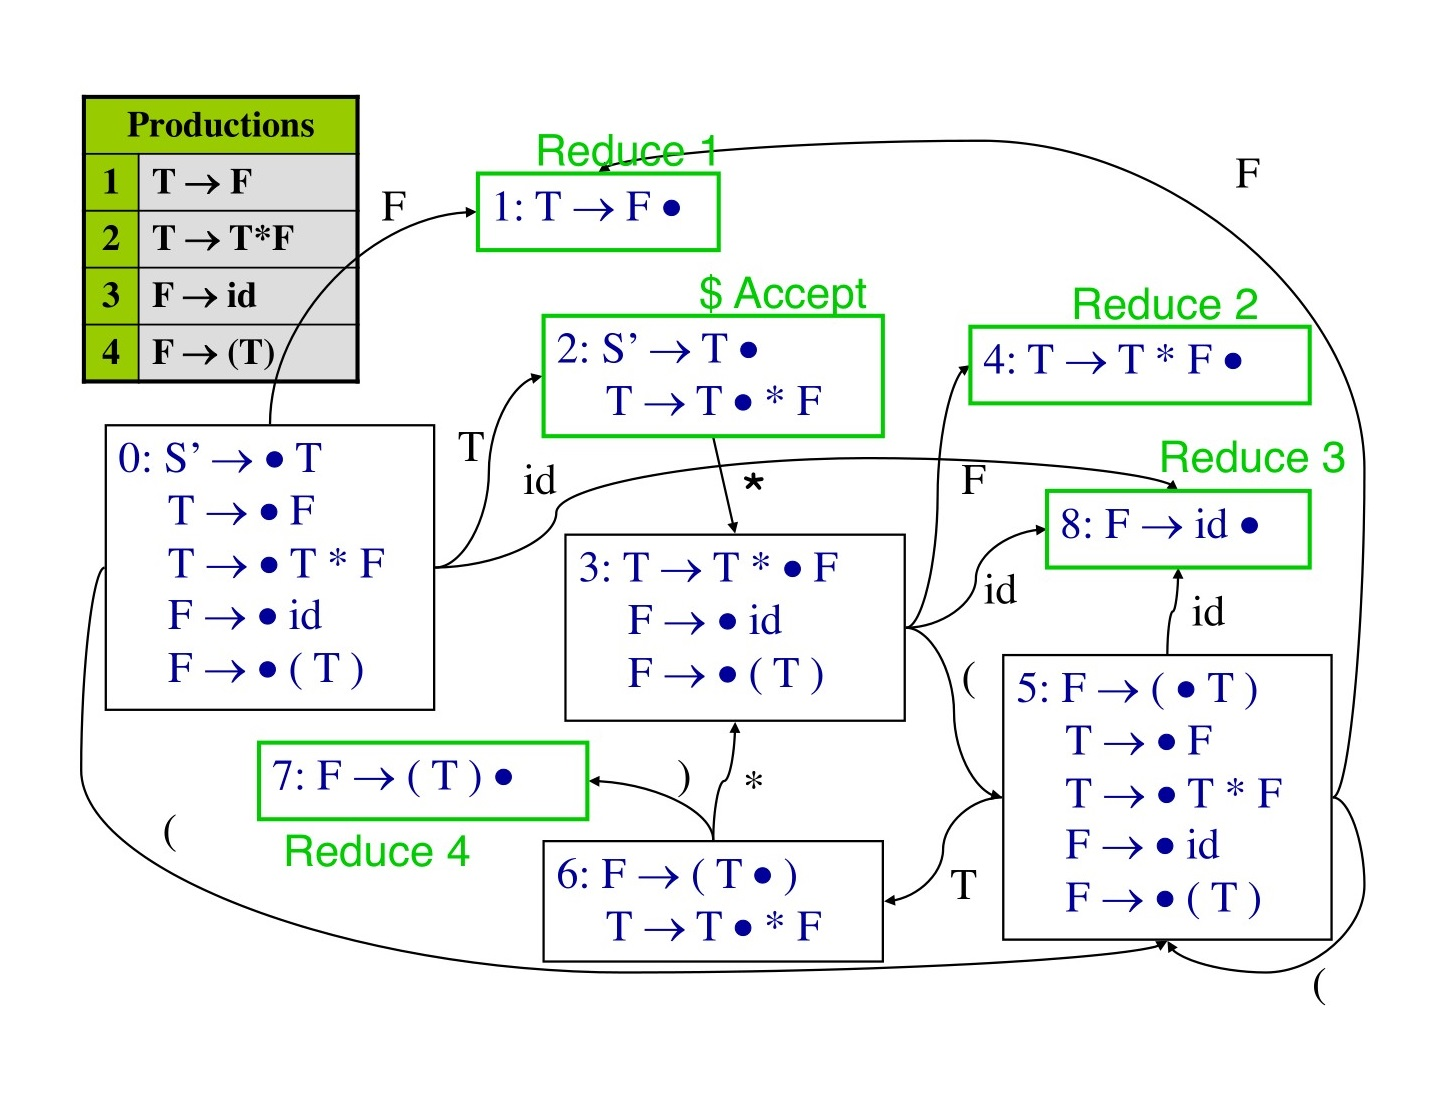
\includegraphics[width=\textwidth]{lrk-states-diagram}
	\end{center}
\end{figure}

	&& For an example diagram of a set of production rules (including epsilon rules) and the states generated using the successor function, see figure~\ref{fig:example-diagram-of-states-epsilon}

\begin{figure}[!htb]
	\caption{Example Diagram of States with Epsilon Rules}
	\label{fig:example-diagram-of-states-epsilon}
	\begin{center}
		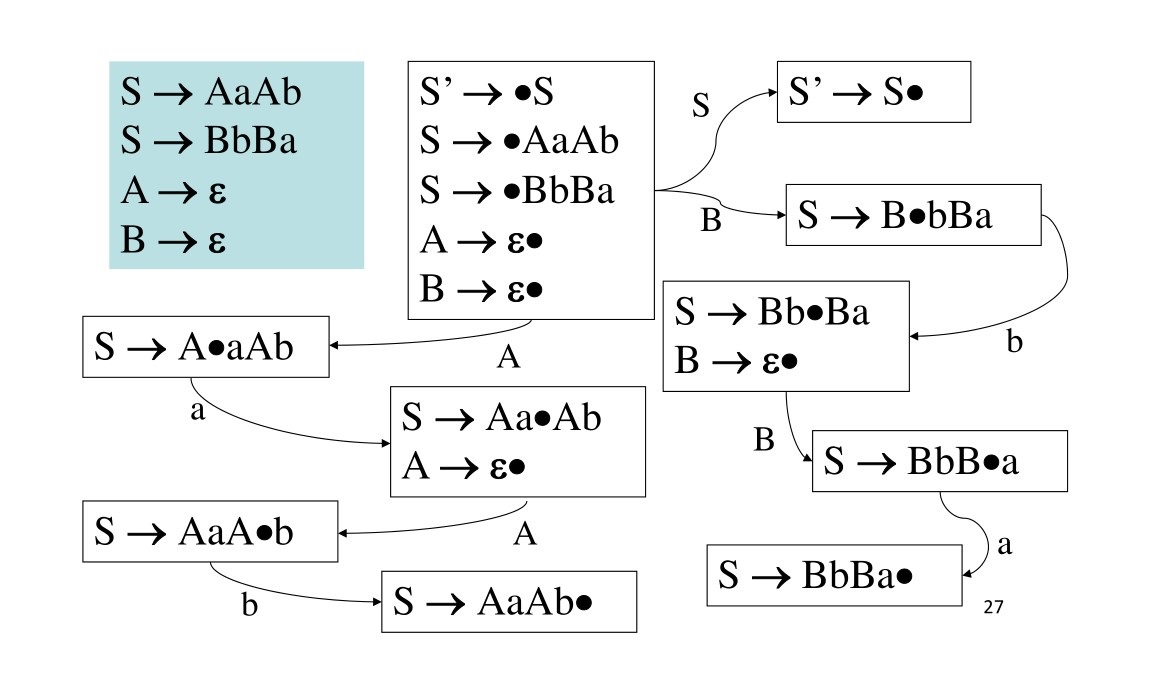
\includegraphics[width=\textwidth]{lrk-states-epsilon-diagram}
	\end{center}
\end{figure}

& \textbf{Viable prefix:} Set of states representing the stack of a shift-reduce parser where combining it with the remaining symbols is a valid state
	&& Notation: $\gamma$ such that $\gamma | \omega$ is a valid state for some $\omega$

& Process of LR(k) parsing:
	&& Requires a set of production rules, an action/goto table, and an input string
	&& Begin with state $0$ on the stack.
	&& From the row number of the current state (given by the top of the stack) and the leftmost symbol in the input, continually take the given action in the action table, given by $\textrm{action}[]$.
		&&& If the action is $S\alpha$, then push state $\alpha$ onto the stack and consume the leftmost symbol of the input.
		&&& If the action is $Rr$, then:
			&&&& Find the production rule numbered $r$, with $r: X \rightarrow Y_1 \dotsc Y_k$.
			&&&& Pop $k$ states from the stack.
			&&&& Take the state $Z$ at the top of the stack and push state $\textrm{goto}[Z, X]$ onto the stack.
		&&& If the action is $\textrm{ACCEPT}$, then complete the parsing.
		&&& If no action exists, then return $\textrm{ERROR}$.

	&& Example: Given the production rules in figure~\ref{tab:lrk-productions} and action/goto table in figure~\ref{tab:lrk-ag-table}, the trace of the LR(0) parse is figure~\ref{tab:lrk-trace}

\end{easylist}
\begin{figure}[!htb]
	\caption{LR(k) Parsing Example: Production Rules}
	\label{tab:lrk-productions}
	\begin{center}
		\begin{tabular}{ r | l }
			& Production Rules \\
			\hline
			1 & $T \rightarrow F$ \\
			2 & $T \rightarrow T*F$ \\
			3 & $F \rightarrow id$ \\
			4 & $F \rightarrow (T)$
		\end{tabular}
	\end{center}
\end{figure}
\begin{easylist}

\end{easylist}
\begin{figure}[!htb]
	\caption{LR(k) Parsing Example: Action/Goto Table}
	\label{tab:lrk-ag-table}
	\begin{center}
		\begin{tabular}{ r | c | c | c | c | c || c | c }
			\multirow{2}{*}{\textbf{States}} & \multicolumn{5}{ c || }{\textbf{Actions}} & \multicolumn{2}{c}{\textbf{Gotos}} \\
			& * & ( & ) & id & \$ & T & F \\
			\hline
			0 & & S5 & & S8 & 2 & 1 \\
			1 & R1 & R1 & R1 & R1 & R1 & \\
			2 & S3 & & & & ACC & \\
			3 & & S5 & & S8 & & 4 \\
			4 & R2 & R2 & R2 & R2 & R2 & \\
			5 & & S5 & & S8 & & 6 & 1 \\
			6 & S3 & & S7 & & & \\
			7 & R4 & R4 & R4 & R4 & R4 & \\
			8 & R3 & R3 & R3 & R3 & R3 &
		\end{tabular}
	\end{center}
\end{figure}
\begin{easylist}

\end{easylist}
\begin{figure}[!htb]
	\caption{LR(k) Parsing Example: Trace}
	\label{tab:lrk-trace}
	\begin{center}
		\begin{tabular}{ l | r | l }
			Stack & Input & Action \\
			\hline
			0 & (id)*id & Shift 5 \\
			0, 5 & id)*id & Shift 8 \\
			0, 5, 8 & )*id & Reduce using production rule 3: $F \rightarrow id$ \\
			&& Pop 1 symbol from the stack (8) \\
			&& Push $goto[5, F] = 1$ onto the stack \\
			0, 5, 1 & )*id & R1: $T \rightarrow F$ \\
			&& Pop 1 \\
			&& $goto[5, T] = 6$ \\
			0, 5, 6 & )*id & S7 \\
			0, 5, 6, 7 & *id & R4, $F \rightarrow (T)$ \\
			&& Pop 7, 6, 5 \\
			&& $goto[0, T] = 1$ \\
			0, 1 & *id & R1: $T \rightarrow F$ \\
			&& Pop 1 \\
			&& $goto[0, T] = 2$ \\
			0, 2 & *id & S3 \\
			0, 2, 3 & id & S8 \\
			0, 2, 3, 8 & \$ & R3: $F \rightarrow id$ \\
			&& Pop 8 \\
			&& $goto]3, F] = 4$ \\
			0, 2, 3, 4 & \$ & R2: $T \rightarrow T*F$ \\
			&& Pop 4, 3, 2 \\
			&& $goto[0, T] = 2$ \\
			0, 2 & \$ & ACCEPT
		\end{tabular}
	\end{center}
\end{figure}
\begin{easylist}

\end{easylist}
\subsection{LR(0) Parsing}
	\label{subsec:parsing-algorithms-bottom-up:lr0}
\begin{easylist}

& \textbf{LR(0) parsing:} Form of LR(k) parsing where no tokens of lookahead are used, so a reduction is always executed whenever possible
	&& \textbf{LR(0) grammar:} Subset of CFGs where an LR(0) construction can be generated without shift-reduce or reduce-reduce conflicts (i.e. the generated pushdown automata is deterministic)

& Grammar validity:
	&& A grammar is LR(0) if and only if no shift-reduce or reduce-reduce conflicts exist in the itemsets
	&& A grammar is not LR(0) if and only if at least one shift-reduce or reduce-reduce conflict exists in the itemsets

\end{easylist}
\subsection{SLR(1) Parsing}
	\label{subsec:parsing-algorithms-bottom-up:slr1}
\begin{easylist}

& \textbf{LR(1) parsing:} Form of LR(k) parsing where 1 token of lookahead is available for use

& \textbf{SLR(1)/SLR/Simple LR parsing:} Subset of LR(0) parsing where each \textit{production rule} includes all possible $FOLLOW$ terminal symbols using 1 character of lookahead

& \textbf{SLR(1)/SLR/Simple LR grammar:} Subset of CFGs where an LR(1) construction can be generated without shift-reduce or reduce-reduce conflicts, or conflicts exist but can be resolved due to having a single $FOLLOW$ symbol
	&& First/follow:
		&&& \textbf{First:} Set of terminal symbols which are the beginning symbols of all strings which can be derived from a given symbol
			&&&& Notation: $FIRST(S) = \{a, b\}$ where $S$ is a given symbol and $a, b$ are terminal symbols
			&&&& Example: Given a set of production rules, the First sets of the non-terminal symbols are derived in table~\ref{tab:first-example}
		&&& \textbf{Follow:} Set of terminal symbols which can follow a given symbol
			&&&& Notation: $FOLLOW(S) = \{a, b\}$ where $S$ is a given symbol and $a, b$ are terminal symbols
			&&&& Example: Given a set of production rules, the Follow sets of the non-terminal symbols are derived in table~\ref{tab:follow-example}
		&&& Example: Given a set of production rules, the First and Follow sets of the non-terminal symbols can be derived as follows:
			&&&& See table~\ref{tab:first-follow-sets-example-1}
			&&&& See table~\ref{tab:first-follow-sets-example-2}

\end{easylist}
\begin{figure}[!htb]
	\caption{First Example}
	\label{tab:first-example}
	\begin{center}
		\begin{tabular}{ r l }
			Production Rules:
			& $A \rightarrow Bc | d$ \\
			& $B \rightarrow e$ \\
			\hline
			$FIRST(A) =$ & $\{d, e\}$ \\
			$FIRST(B) =$ & $\{e\}$
		\end{tabular}
	\end{center}
\end{figure}
\begin{easylist}

\end{easylist}
\begin{figure}[!htb]
	\caption{Follow Example}
	\label{tab:follow-example}
	\begin{center}
		\begin{tabular}{ r l }
			Production Rules:
			& $A \rightarrow Bc$ \\
			& $B \rightarrow Bd | BC$ \\
			& $C \rightarrow e$ \\
			\hline
			$FOLLOW(A) =$ & $\{ \$ \}$ \\
			$FOLLOW(B) =$ & $\{c, d, e\}$ \\
			$FOLLOW(C) =$ & $\{c\}$
		\end{tabular}
	\end{center}
\end{figure}
\begin{easylist}

\end{easylist}
\begin{figure}[!htb]
	\caption{First/Follow Sets Example 1}
	\label{tab:first-follow-sets-example-1}
	\begin{center}
		\begin{tabular}{ r | l }
			Production Rules
			& $S \rightarrow AB$ \\
			& $A \rightarrow c | \epsilon$ \\
			& $B \rightarrow cbB | a$ \\
			\hline
			First sets
			& $FIRST(A) = \{c, \epsilon\}$ \\
			& $FIRST(B) = \{c, a\}$ \\
			& $FIRST(S) = FIRST(A) = \{c, \epsilon\}$ \\
			\hline
			Follow sets
			& $FOLLOW(A) = FIRST(B) = \{c, a\}$ \\
			& $FOLLOW(B) = \{\$\}$ \\
			& $FOLLOW(S) = \{\$\}$
		\end{tabular}
	\end{center}
\end{figure}
\begin{easylist}

\end{easylist}
\begin{figure}[!htb]
	\caption{First/Follow Sets Example 2}
	\label{tab:first-follow-sets-example-2}
	\begin{center}
		\begin{tabular}{ r | l }
			Production Rules
			& $S \rightarrow cAa$ \\
			& $A \rightarrow cB | B$ \\
			& $B \rightarrow bcB | \epsilon$ \\
			\hline
			First sets
			& $FIRST(A) = \{c, b, \epsilon\}$ \\
			& $FIRST(B) = \{b, \epsilon\}$ \\
			& $FIRST(S) = \{c\}$ \\
			\hline
			Follow sets
			& $FOLLOW(A) = \{a\}$ \\
			& $FOLLOW(B) = FOLLOW(A) = \{a\}$ \\
			& $FOLLOW(S) = \{\$\}$
		\end{tabular}
	\end{center}
\end{figure}
\begin{easylist}

	&& Process to determine whether a shift-reduce conflict can be eliminated by a 1-token lookahead:
		&&& Find the $FOLLOW$ set of the reduce rule
		&&& Find the next accepted symbol of the shift rule
		&&& If the symbol is in the $FOLLOW$ set, then the conflict cannot be eliminated
		&&& Example: Given the set of production rules in table~\ref{tab:slr-shift-reduce}, the state $S \rightarrow A \bullet xB; B \rightarrow A \bullet$ has a shift-reduce conflict which cannot be resolved by 1 token of lookahead, as the parser can still shift or reduce on $x$ because the $FOLLOW$ set of $B$ is $\{ x, \$ \}$

\end{easylist}
\begin{figure}[!htb]
	\caption{SLR Shift-Reduce Conflict Example}
	\label{tab:slr-shift-reduce}
	\begin{center}
		\begin{tabular}{ l }
			$S \rightarrow Ax$ \\
			$S \rightarrow B$ \\
			$B \rightarrow A$ \\
			$A \rightarrow yB$
		\end{tabular}
	\end{center}
\end{figure}
\begin{easylist}

	&& Example: Given the set of production rules and transition diagram in figure~\ref{fig:slr-1-parsing-prod-rules-diagram}, the trace of the SLR(1) parse of $id * id$ is table~\ref{tab:slr-1-parsing-trace}

\begin{figure}[!htb]
	\caption{SLR(1) Parsing Example: Production Rules and Diagram}
	\label{fig:slr-1-parsing-prod-rules-diagram}
	\begin{center}
		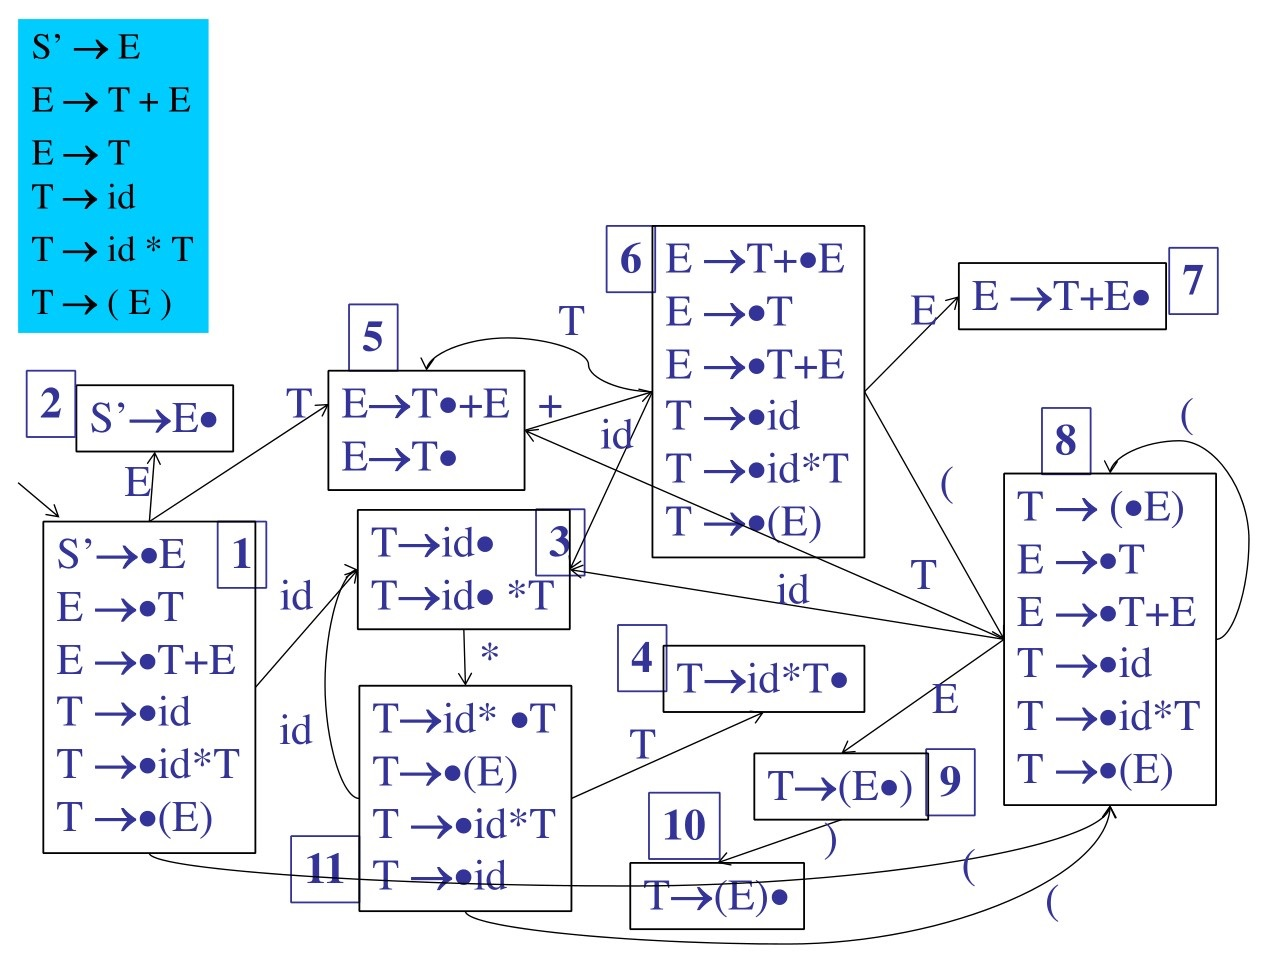
\includegraphics[width=\textwidth]{slr-1-trace-diagram}
	\end{center}
\end{figure}

\end{easylist}
\begin{figure}[!htb]
	\caption{SLR(1) Parsing Example: Trace}
	\label{tab:slr-1-parsing-trace}
	\begin{center}
		\begin{tabular}{ l | r | l }
			Stack and Input & DFA Halt State & Action \\
			\hline
			$| id * id\$ $ & $1$ & Shift \\
			$id | * id\$ $ & $3 ( \* \not\in FOLLOW(T) )$ & Shift \\
			$id * | id\$ $ & $11$ & Shift \\
			$id * id |\$ $ & $3 (\$ \in FOLLOW(T) )$ & Reduce $T \rightarrow id$ \\
			$id * T | \$ $ & $4 (\$ \in FOLLOW(T) )$ & Reduce $T \rightarrow id * T$ \\
			$T | \$ $ & $5 (\$ \in FOLLOW(T) )$ & Reduce $E \rightarrow T$ \\
			$E | \$ $ & & Accept
		\end{tabular}
	\end{center}
\end{figure}
\begin{easylist}

& Grammar validity:
	&& A grammar is SLR(1) if and only if, for each shift-reduce or reduce-reduce conflict in the configuration sets, the $FOLLOW$ sets of the conflicting production rules (not dotted rules) do not intersect
	&& A grammar is not SLR(1) if and only if there exists at least one shift-reduce or reduce-reduce conflict in the configuration sets where the $FOLLOW$ sets of the conflicting production rules intersect

\end{easylist}
\subsection{Canonical LR(1) Parsing}
	\label{subsec:parsing-algorithms-bottom-up:canonical-lr1}
\begin{easylist}

& \textbf{LR(1)/Canonical LR(1) parsing:} Subset of LR(0) parsing where each \textit{dotted rule} includes a 1-character lookahead, rather than each production rule
	&& More accurate than SLR(1) parsing
	&& Notation: $\textrm{dotted rule, } \alpha / \beta$ where $\alpha, \beta$ are the potential $FOLLOW$ characters of the non-terminal symbol if the rule was parsed and reduced
	
& Grammar validity:
	&& A grammar is LR(1) if and only if, for each shift-reduce or reduce-reduce conflict, the $FOLLOW$ sets of the dotted rules do not conflict
	&& A grammar is not LR(1) if and only if there exists at least one itemset where conflicting dotted rules have intersecting $FOLLOW$ sets

\end{easylist}
\subsection{LALR(1) Parsing}
	\label{subsec:parsing-algorithms-bottom-up:lalr1}
\begin{easylist}

& \textbf{LALR(1) parsing:} Subset of LR(0) parsing which combines states when they share the same dotted rules but have different $FOLLOW$ sets
	&& More specific than SLR(1) (as resulting $FOLLOW$ sets may not always be the complete \\ $FOLLOW$ set)
	&& Simplified/compact version of canonical LR(1)
	
& Grammar validity:
	&& A grammar is LALR(1) if and only if, when states with matching dotted rules are merged, for each combination of states, for each matching dotted rule in the resulting configuration set, there are no conflicts in the 1-character lookaheads
	&& A grammar is not LALR(1) if and only if, when states with matching dotted rules are merged, the $FOLLOW$ sets contain shift-reduce or reduce-reduce conflicts

\end{easylist}
\clearpage
